\section{Results}
\label{sec:results}
\subsection{Frequency of Regex \emph{Utilizations} in Python Projects}
\subsubsection{Saturation of Projects with Regex \emph{Utilizations}}
Out of the \DTLfetch{data}{key}{nProjScanned}{value}\ projects scanned, \DTLfetch{data}{key}{percentProjectsUsingRegex}{value}\% (\DTLfetch{data}{key}{nProjectsUsingRegex}{value}) contained at least one \emph{utilization}.  For context about how saturated these projects were with regex \emph{utilizations}, we consider how many files the average project scanned contained, how many of those files contained \emph{utilizations}, and how many \emph{utilizations} occurred per file in table~\ref{table:contextHistogram}.

\begin{table}[tb]
\centering
\begin{center}
\begin{tabular}{l|ccccc}
\toprule
source & Q1 & Avg & Med & Q3 & Max \\ 
\midrule
files per project & 2 & 53 & 6 & 21 & 5,963 \\ 
\midrule
files with regex per project & 1 & 11 & 2 & 6 & 541 \\ 
\midrule
regex usages per file & 1 & 2 & 1 & 3 & 207 \\ 
\bottomrule
\end{tabular}
\end{center}

\caption{How saturated are projects with \emph{utilizations}? (RQ1)}
\label{table:contextHistogram}
\end{table}

\subsubsection{Usage Frequency of {\tt re} Module Functions and Flags}

\begin{figure}[tb]
\centering
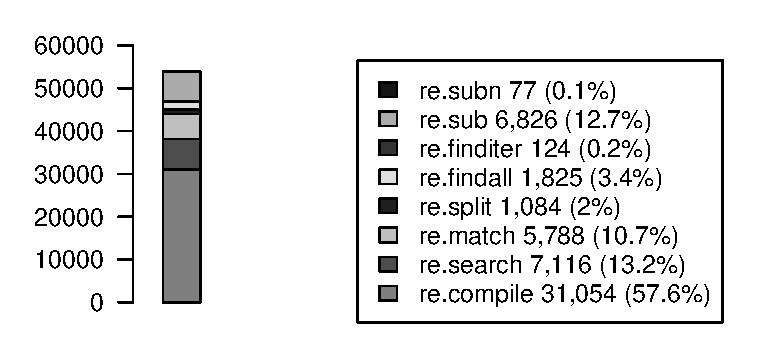
\includegraphics[width=\columnwidth]{../analysis_output/partFunctions.eps}
\caption{How often are the 8 re functions used? (RQ1)}
\label{fig:partFunctions}
\end{figure}

As seen in Figure~\ref{fig:partFunctions} The `compile' function encompasses \DTLfetch{data}{key}{percentCompile}{value}\% of all \emph{utilizations}, presumably because each usage of those functions could accept the compiled regex as an argument.

\begin{figure}[tb]
\centering
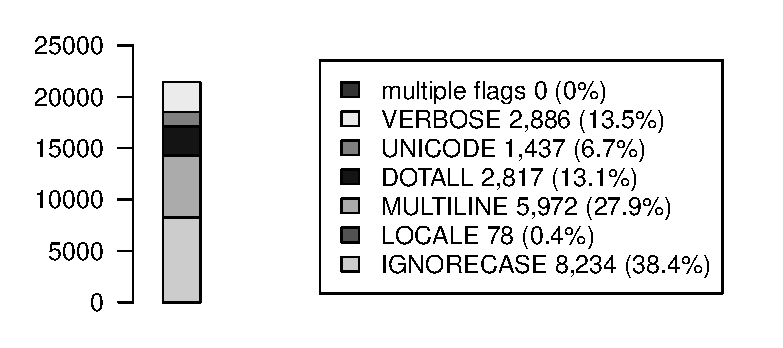
\includegraphics[width=\columnwidth]{../analysis_output/partFlags.eps}
\caption{Which behavioral flags are used? (RQ1)}
\label{fig:partFlags}
\end{figure}

When considering flag use, we excluded non-behavioral flags (default and debug), which account for \DTLfetch{data}{key}{percentFlags0}{value}\% of all \emph{utilizations}.

 As shown in figure ~\ref{fig:partFlags}, of all behavioral flags used, ignorecase (\DTLfetch{data}{key}{percentI}{value}\%) and multiline (\DTLfetch{data}{key}{percentM}{value}\%) were the most frequently used.  It is also worth noting that although multiple flags can be combined using a bitwise or, this was never observed.

\todo{topNW table?}
% \subsubsection{{General Characteristics of Regexes Found}}
% \todo{could the top 10 regexes be a pop-out?}
% \begin{table}
\caption{ \label{}}
\begin{center}
\begin{tabular}{lc}
\toprule
pattern & weight \\ 
\midrule
\begin{minipage}{2.3in}
\begin{verbatim}
'\\s+'\end{verbatim}
\end{minipage}
& 181 \\ 
\midrule
\begin{minipage}{2.3in}
\begin{verbatim}
'\\s'\end{verbatim}
\end{minipage}
& 78 \\ 
\midrule
\begin{minipage}{2.3in}
\begin{verbatim}
'\\d+'\end{verbatim}
\end{minipage}
& 70 \\ 
\midrule
\begin{minipage}{2.3in}
\begin{verbatim}
'[\\x80-\\xff]'\end{verbatim}
\end{minipage}
& 69 \\ 
\midrule
\begin{minipage}{2.3in}
\begin{verbatim}
'\nmd5_data = {\n([^}]+)}'\end{verbatim}
\end{minipage}
& 69 \\ 
\midrule
\begin{minipage}{2.3in}
\begin{verbatim}
'\\\\(.)'\end{verbatim}
\end{minipage}
& 67 \\ 
\midrule
\begin{minipage}{2.3in}
\begin{verbatim}
'([\\\\"]|[^\\ -~])'\end{verbatim}
\end{minipage}
& 66 \\ 
\midrule
\begin{minipage}{2.3in}
\begin{verbatim}
'(-?(?:0|[1-9]\\d*))(\\.\\d+)?([eE][-+]?\\d+)?'\end{verbatim}
\end{minipage}
& 61 \\ 
\midrule
\begin{minipage}{2.3in}
\begin{verbatim}
'[^]]+?\\] +([0-9.]+): (\\w+) <-(\\w+)'\end{verbatim}
\end{minipage}
& 60 \\ 
\midrule
\begin{minipage}{2.3in}
\begin{verbatim}
'.*rlen=([0-9]+)'\end{verbatim}
\end{minipage}
& 57 \\ 
\bottomrule
\end{tabular}
\end{center}
\end{table}


\subsection{Frequency of Feature Usage}

Literal tokens were found in \DTLfetch{data}{key}{P_LITERAL_PRESENT}{value}\% of patterns, and accounted for \DTLfetch{data}{key}{P_LITERAL_TOKENS}{value}\% of all tokens.  We consider literal tokens to be ubiquitous in all \emph{utilizations}, and necessary for any regex related tool, and so exclude them from the rest of the feature analysis.  In table~\ref{table:featureStats}, we display a large body of information about feature usage and relate it to four major regex related projects.

\begin{table*}[h]
\begin{center}
\begin{small}
\caption{How Frequently do Features Appear in Projects? (RQ2)}
\label{table:featureStats}
\begin{tabular}
{ll@{ }llc@{ }c@{ }c@{ }ccccccc}
rank & code & description & example & brics & hampi & Rex & RE2 & nPatterns & \% patterns & nProjects & \% projects \\ 
\toprule[0.16em]
1 & ADD & one-or-more repetition & \begin{minipage}{0.5in}\begin{verbatim}z+\end{verbatim}\end{minipage} & \yes & \yes & \yes & \yes & 6,003 & 44.1 & 1,204 & 73.2 \\ 
\midrule
2 & CG & a capture group & \begin{minipage}{0.5in}\begin{verbatim}(caught)\end{verbatim}\end{minipage} & \yes & \yes & \yes & \yes & 7,130 & 52.4 & 1,194 & 72.6 \\ 
\midrule
3 & KLE & zero-or-more repetition & \begin{minipage}{0.5in}\begin{verbatim}.*\end{verbatim}\end{minipage} & \yes & \yes & \yes & \yes & 6,017 & 44.3 & 1,099 & 66.8 \\ 
\midrule
4 & CCC & custom character class & \begin{minipage}{0.5in}\begin{verbatim}[aeiou]\end{verbatim}\end{minipage} & \yes & \yes & \yes & \yes & 4,468 & 32.9 & 1,026 & 62.4 \\ 
\midrule
5 & ANY & any non-newline char & \begin{minipage}{0.5in}\begin{verbatim}.\end{verbatim}\end{minipage} & \yes & \yes & \yes & \yes & 4,657 & 34.3 & 1,005 & 61.1 \\ 
\midrule
6 & RNG & chars within a range & \begin{minipage}{0.5in}\begin{verbatim}[a-z]\end{verbatim}\end{minipage} & \yes & \yes & \yes & \yes & 2,631 & 19.3 & 848 & 51.6 \\ 
\midrule
7 & STR & start-of-line & \begin{minipage}{0.5in}\begin{verbatim}^\end{verbatim}\end{minipage} & \no & \yes & \yes & \yes & 3,563 & 26.2 & 846 & 51.4 \\ 
\midrule
8 & END & end-of-line & \begin{minipage}{0.5in}\begin{verbatim}$\end{verbatim}\end{minipage} & \no & \yes & \yes & \yes & 3,169 & 23.3 & 827 & 50.3 \\ 
\midrule[0.12em]
9 & NCCC & negated CCC & \begin{minipage}{0.5in}\begin{verbatim}[^qwxf]\end{verbatim}\end{minipage} & \yes & \yes & \yes & \yes & 1,935 & 14.2 & 776 & 47.2 \\ 
\midrule
10 & WSP & \textbackslash t \textbackslash n \textbackslash r \textbackslash v \textbackslash f or space & \begin{minipage}{0.5in}\begin{verbatim}\s\end{verbatim}\end{minipage} & \no & \yes & \yes & \yes & 2,846 & 20.9 & 762 & 46.3 \\ 
\midrule
11 & OR & logical or & \begin{minipage}{0.5in}\begin{verbatim}a|b\end{verbatim}\end{minipage} & \yes & \yes & \yes & \yes & 2,102 & 15.5 & 708 & 43 \\ 
\midrule
12 & DEC & any of: 0123456789 & \begin{minipage}{0.5in}\begin{verbatim}\d\end{verbatim}\end{minipage} & \no & \yes & \yes & \yes & 2,297 & 16.9 & 692 & 42.1 \\ 
\midrule
13 & WRD & [a-zA-Z0-9\_] & \begin{minipage}{0.5in}\begin{verbatim}\w\end{verbatim}\end{minipage} & \no & \yes & \yes & \yes & 1,430 & 10.5 & 650 & 39.5 \\ 
\midrule
14 & QST & zero-or-one repetition & \begin{minipage}{0.5in}\begin{verbatim}z?\end{verbatim}\end{minipage} & \yes & \yes & \yes & \yes & 1,871 & 13.8 & 645 & 39.2 \\ 
\midrule
15 & LZY & as few reps as possible & \begin{minipage}{0.5in}\begin{verbatim}z+?\end{verbatim}\end{minipage} & \no & \yes & \no & \yes & 1,300 & 9.6 & 605 & 36.8 \\ 
\midrule
16 & NCG & group without capturing & \begin{minipage}{0.5in}\begin{verbatim}a(?:b)c\end{verbatim}\end{minipage} & \no & \yes & \no & \yes & 791 & 5.8 & 404 & 24.6 \\ 
\midrule
17 & PNG & named capture group & \begin{minipage}{0.5in}\begin{verbatim}(?P<name>x)\end{verbatim}\end{minipage} & \no & \yes & \no & \yes & 915 & 6.7 & 354 & 21.5 \\ 
\midrule
18 & SNG & exactly n repetition & \begin{minipage}{0.5in}\begin{verbatim}z{8}\end{verbatim}\end{minipage} & \yes & \yes & \yes & \yes & 581 & 4.3 & 340 & 20.7 \\ 
\midrule
19 & NWSP & any non-whitespace & \begin{minipage}{0.5in}\begin{verbatim}\S\end{verbatim}\end{minipage} & \no & \yes & \yes & \yes & 484 & 3.6 & 270 & 16.4 \\ 
\midrule
20 & DBB & $n\le x \le m$ repetition & \begin{minipage}{0.5in}\begin{verbatim}z{3,8}\end{verbatim}\end{minipage} & \yes & \yes & \yes & \yes & 367 & 2.7 & 238 & 14.5 \\ 
\midrule
21 & NLKA & sequence doesn't follow  & \begin{minipage}{0.5in}\begin{verbatim}a(?!yz)\end{verbatim}\end{minipage} & \no & \no & \no & \no & 131 & 1 & 183 & 11.1 \\ 
\midrule
22 & WNW & word/non-word boundary & \begin{minipage}{0.5in}\begin{verbatim}\b\end{verbatim}\end{minipage} & \no & \no & \no & \yes & 248 & 1.8 & 166 & 10.1 \\ 
\midrule
23 & NWRD & non-word chars & \begin{minipage}{0.5in}\begin{verbatim}\W\end{verbatim}\end{minipage} & \no & \yes & \yes & \yes & 94 & 0.7 & 165 & 10 \\ 
\midrule
24 & LWB & at least n repetition & \begin{minipage}{0.5in}\begin{verbatim}z{15,}\end{verbatim}\end{minipage} & \yes & \yes & \yes & \yes & 91 & 0.7 & 158 & 9.6 \\ 
\midrule
25 & LKA & matching sequence follows & \begin{minipage}{0.5in}\begin{verbatim}a(?=bc)\end{verbatim}\end{minipage} & \no & \no & \no & \no & 112 & 0.8 & 158 & 9.6 \\ 
\midrule
26 & OPT & options wrapper & \begin{minipage}{0.5in}\begin{verbatim}(?i)CasE\end{verbatim}\end{minipage} & \no & \yes & \no & \yes & 231 & 1.7 & 154 & 9.4 \\ 
\midrule
27 & NLKB & sequence doesn't precede & \begin{minipage}{0.5in}\begin{verbatim}(?<!x)yz\end{verbatim}\end{minipage} & \no & \no & \no & \no & 94 & 0.7 & 137 & 8.3 \\ 
\midrule[0.12em]
28 & LKB & matching sequence precedes & \begin{minipage}{0.5in}\begin{verbatim}(?<=a)bc\end{verbatim}\end{minipage} & \no & \no & \no & \no & 80 & 0.6 & 120 & 7.3 \\ 
\midrule
29 & ENDZ & absolute end of string & \begin{minipage}{0.5in}\begin{verbatim}\Z\end{verbatim}\end{minipage} & \no & \no & \no & \yes & 89 & 0.7 & 90 & 5.5 \\ 
\midrule
30 & BKR & match the $i^{th}$ CG & \begin{minipage}{0.5in}\begin{verbatim}\1\end{verbatim}\end{minipage} & \no & \no & \no & \no & 60 & 0.4 & 84 & 5.1 \\ 
\midrule
31 & NDEC & any non-decimal & \begin{minipage}{0.5in}\begin{verbatim}\D\end{verbatim}\end{minipage} & \no & \yes & \yes & \yes & 36 & 0.3 & 58 & 3.5 \\ 
\midrule
32 & BKRN & references PNG & \begin{minipage}{0.5in}\begin{verbatim}\g<name>\end{verbatim}\end{minipage} & \no & \yes & \no & \no & 17 & 0.1 & 28 & 1.7 \\ 
\midrule
33 & VWSP & matches U+000B & \begin{minipage}{0.5in}\begin{verbatim}\v\end{verbatim}\end{minipage} & \no & \no & \yes & \yes & 13 & 0.1 & 15 & 0.9 \\ 
\midrule
34 & NWNW & negated WNW & \begin{minipage}{0.5in}\begin{verbatim}\B\end{verbatim}\end{minipage} & \no & \no & \no & \yes & 4 & 0 & 11 & 0.7 \\ 
\bottomrule[0.13em]
\end{tabular}
\end{small}
\end{center}
\vspace{-12pt}
\end{table*}

%note captions and label are in external file
% use:\label{table:featureStats}

\subsection{What Features Are Used For}


% TODO - multiple boxplots for all 5-6 demonstrating cluster size and then also have \# of clusters, pick smallest number of clusters and then use that.






